\subsection{Method}
In this section the methodology is covered in four parts.
First the practical procedure chosen in this work for applying spectral clustering is given.
Secondly, choices and interpretations for the variable parameters in this algorithm are given.
Then the datasets against which this will be measured are specified.
Finally the procedure for checking infrared-collinear (IRC) safety will be described.


\subsubsection{Clustering algorithm}\label{sec:spectralmethodalgo}
    The implementation of the theory described in section~\ref{sec:spectral_theory} will be specified.
    For every simulated event this process if used to identify the jets.

    \begin{enumerate}
        \item \label{step:start} The particles will be used to form the nodes of a graph,
        the edges of which will be weighted by some measure of proximity between the particles called affinity.
        To obtain an affinity, first a distance is obtained; \(d_{i,j} = \sqrt{(y_i - y_j)^2 + (\phi_i - \phi_j)^2}\)
        where \(y_i\) is the rapidity of particle \(i\) and \(\phi_i\) is the barrel angle is particle \(i\).
        No \(p_T\) dependence is used.

    \item \label{step:affinity} The affinity must increase as particles become more similar, whereas the distance will shrink.
            This is done by taking an exponent so that \(a_{i,j} = \text{exp}(-d_{i,j}^\alpha/\sigma)\), as done in~\cite{hadjighasem2016votex}. % TODO check you stick with this
            %Sigma (\(\sigma\)) defines a scale for the distances.
            Distances much larger than \(\sigma\) are only allowed very small affinities,
            thus less influence over the clustering.
            %It is tunable and chosen to be \(0.2\).
    \item\label{step:KNN} The affinity between particles that are far apart contains less useful information,
        such particles are unlikely to be genuinely related.
        Removing these affinities reduces noise.
    A fixed number, \(k_\text{NN}\), of neighbours of each point are
    preserved, and all other affinities are set to zero.

\item\label{step:laplacean} These affinities allow the construction of a Laplacian.
        The Laplacian used is the symmetric Laplacien, which has \(-a_{i,j}/(\sum_k a_{i,k})^{0.5}(\sum_k a_{j,k})^{0.5}\)
        in the \(i\)th row and \(j\)th column, and \(1\) all along the diagonal.
        The two factors in the denominator, \((\sum_k a_{i, k})^{0.5}\) and \((\sum_k a_{j, k})^{0.5}\) are the weights of \(i\) and \(j\).
        In subsequent iterations weights will not be recalculated,
        if a particle is combined with another particle, the weight of the new object is the sum of the weights of the old objects.
        This condition is required for IRC safety.
        Let \(z_i = \sum_k a_{i,k}\), then
    \begin{equation}\label{eqn:laplacian}
        L = 
        \begin{pmatrix}
            z_0      & 0   & 0  & \hdots \\
               0     & z_1 &    0     & \\
               0     &    0     & z_2 & \\
            \vdots   &          &     & \ddots 
        \end{pmatrix}^{-\frac{1}{2}}
        \begin{pmatrix}
            z_0 & -a_{0,1} & -a_{0,2} & \hdots \\
            -a_{0,1} & z_1 & -a_{1,2} & \\
            -a_{0,2} & -a_{1,2} & z_2 & \\
            \vdots   &          &     & \ddots 
        \end{pmatrix}
        \begin{pmatrix}
            z_0 &    0     &    0     & \hdots \\
               0     & z_1 &    0     & \\
               0     &    0     & z_2 & \\
            \vdots   &          &     & \ddots 
        \end{pmatrix}^{-\frac{1}{2}}.
    \end{equation}

\item \label{step:eigenvectors} From the Laplacian eigenvectors are calculated to create the embedding space.
            All eigenvectors corresponding to an eigenvalue less that the eigenvalue limit, \(\lambda_\text{limit}\), are considered.
        The eigenvectors have as many elements as there are particles, and the coordinates of
        the \(i\)th particle in the embedding space is the \(i\)th element of each eigenvector.

    \item \label{step:compression} Each coordinate direction is divided by the corresponding eigenvalue raised to \(\lambda_\text{exponent}\).
            %in this case \(1.5\). 
            This acts to compress the dimensions that hold less information.

        \item \label{step:stoppingcondition} The distance between all objects in the embedding space is calculated.
            Provided the mean of this distance is less than \stoppingdeltar{} then
        the two objects that have the smallest embedding distance are combined.
        %The value of \stoppingdeltar{} used here is \(1.26\).
        In physical space the combined object is created by summing the respective four momenta,
        in the embedding space two methods for locating the combined object are tried.
        Once two objects have been combined in physical space, the embedding space is recalculated from step~\ref{step:start},
        with the caveat mentioned in step~\ref{step:laplacean} that weights are not recalculated.
        %\begin{enumerate}
        %    \item In a \spectralmeanjet{} clustering the location of the combined object is the
        %    geometric mean of the inputs. The clustering then continues to combine things in this manner.
        %    This method has been abandoned as it sculpted the PT distribution.
        %\item \label{fullmethod} In a \spectralfulljet{} once two objects have been combined in physical space,
        %        the embedding space is recalculated from step~\ref{step:start}. 
        %\end{enumerate}
        %In this instance only \ref{fullmethod} is used.


    \item When the mean of the distances in the embedding space rises above \stoppingdeltar{},
        then all objects are promoted to jets. Jets with less than 2 tracks are removed,
        and their contents considered noise,
        as are jets that do not pass \(p_T\) cuts.
    \end{enumerate}
    To provide a basis for comparison the results of clustering with an anti-kt algorithm (as in~\cite{Cacciari2008akt}) is also shown.

\subsubsection{Tunable parameters}\label{sec:spectralmethodparam}
Unlike most machine learning techniques, Spectral clustering does not have large arrays of learnt parameters.
The parameters for the clustering are a small, interpretable, set.
Appropriate values were chosen by performing scans and observing the influence of changes to the parameters on jets formed.

In section~\ref{sec:spectralmethodalgo} 5 parameters are named;
\(\sigma\), \(\alpha\), \(k_\text{NN}\), \(\lambda_\text{limit}\), \(\lambda_\text{exponent}\) and \stoppingdeltar{}.
These parameters have a range of values for which sensible results are obtained.
The interpretation of these parameters is given here;
\begin{itemize}
    \item \(\sigma\); introduced in step~\ref{step:affinity}, this is a scale parameter in physical space.
                      The value indicated an approximate distance within which particles are deemed close.
                      The value used here is \(\sigma = 0.15)\).
    \item  \(\alpha\); also introduced in step~\ref{step:affinity}, this controls the rate which which 
           the influence of particles further away drops. 
           Higher values increase how strictly the parameter \(\sigma\) is used to define a neighbourhood.
          % The value used here is \(\alpha = 1.4\).
       \item \(k_\text{NN}\); introduced in step~\ref{step:KNN}, this dictates the minimum number of non-zero affinities around each point.
           Lower values create a sparser affinity matrix, reducing noise at the potential cost of lost signal.
       \item  \(\lambda_\text{limit}\); introduced in step~\ref{step:eigenvectors}, is a means of limiting the number of eigenvectors used
           to create dimensions in the embedding space.
           The eigenvalue associated with an eigenvector determines the quality of the information it contains about the allocation of points to clusters,
           lower values indicate better information.
           Only eigenvectors corresponding to eigenvalues less than \(\lambda_\text{limit}\) are used.
          % The value chosen here is \(\lambda_\text{limit} = 0.4\).
       \item  \(\lambda_\text{exponent}\); is introduced in step~\ref{step:compression}.
           To account for variable quality of information in the eigenvectors, as given by their eigenvalues,
        dimensions of the embedding space with lower quality information are compressed.
        Quality of information is proportionate of the size of the eigenvalue, o the correct compression is found by
        dividing the lengths in the dimension by \(\lambda^{\lambda_\text{exponent}}\).
        The larger the value of \(\lambda_\text{exponent}\) the more dimensions with lower quality information are compressed.
      %  The value chosen here is \(\lambda_\text{exponent} = 1.6\).
    \item \stoppingdeltar{}; is introduced in step~\ref{step:stoppingcondition}.
         This determines the expected spacing between jets. 
         Of all the parameters this one may be most process specific.
      %   The value selected here is \(\stoppingdeltar{} = 1.26\).
\end{itemize}


A number of other parameters that could influence clustering were experimented with,
including changed of Laplacian and parameters using \(p_T\).
These modifications did not seem to improve performance, so they are not included.

To investigate the behaviour of the clustering when the parameters change scans where performed.
On a small sample of events (\(2\)k events) the clustering is performed with many different parameter choices.

With the aid of MC truth information a metric of success can be created.
For each object we wish to find (e.g. a \bthing{quark}) 
the MC truth can reveal which of the particles that are visible to the detector have
been created by that object.
In many cases, a particle see in the detector will have been created by two objects,
such as a particle coming from an interaction between a \(b-\bar{b}\) pair,
in these cases both objects are considered together.
The complete set of visible particles that came from these objects could be referred to as their descendants.
The aim in jet clustering is to capture only all of the descendants in the same number of jets as there were objects that created them.
So the descendants of \(b-\bar{b}\) pair should be captured in exactly 2 jets.

There are two ways a jet finding algorithm can make mistakes in this task:
the first is to omit some of the descendants of the objects being reconstructed, causing the jet to have less mass than it should;
the second is to include particles that are not in the descendants of the objects being reconstructed, such as initial state radiation or particles from other objects,
causing the jet to have more mass than it should.
The effects of these mistakes will cancel in the jet mass,
but they are both still individually undesirable,
so separate metrics are made for each of them.
The first is ``Signal mass lost", the mass of all descendants of the object being reconstructed that were not included in the jet.
The second is ``Background contamination", the mass of particles included in the jet that are not descendants of the objects being reconstructed.
The standard algorithm for this process, the Anti-KT algorithm with \(\stoppingdeltar{}=0.8\), slightly prefers suppressing ``Signal mass lost" over ``Background contamination",
this leads to the clearest mass peaks.
When the metrics are combined into a single loss value this is accounted for by weighting;
\begin{equation}\label{eqn:loss}
\text{Loss} = \sqrt{0.73(\text{Background contamination})^2 + (\text{Signal mass lost})^2}
\end{equation}

An example of this scan for the generalised KT algorithm is given in figure~\ref{fig:scan_genkt}.
For spectral clustering there are more than 2 variables to deal with, 
so a set of two dimensional slices are shown in figure
These slices have been chosen to include the best performing combination.
    \begin{figure}[htp]
        \begin{minipage}[c]{0.5\textwidth}
            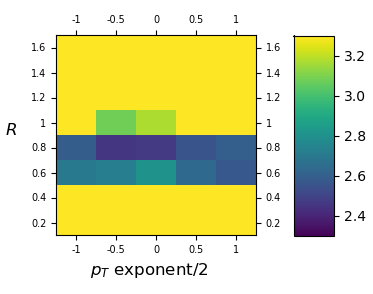
\includegraphics[width=1\textwidth]{graphics/trangle_scan_genkt.png}
        \end{minipage}\hfill
        \begin{minipage}[c]{0.45\textwidth}
            \caption{Generalised-KT algorithm offers two parameters that can be varied.
                The stopping condition, \stoppingdeltar{}, and a multiple for the exponent of the \(p_T\) factor.
                When the exponent of the \(p_T\) factor is \(-1\) the algorithm becomes the Anti-KT algorithm.
                Here the loss, as described in equation~\ref{eqn:loss}, is shown for a number of parameter combinations.
                It can be seen that while good results are possible with many values of \(p_T\) exponent,
                \stoppingdeltar{} must fall in a narrow range to yield good results.
             }\label{fig:scan_genkt}
        \end{minipage}
    \end{figure}    

    \begin{figure}[htp]
            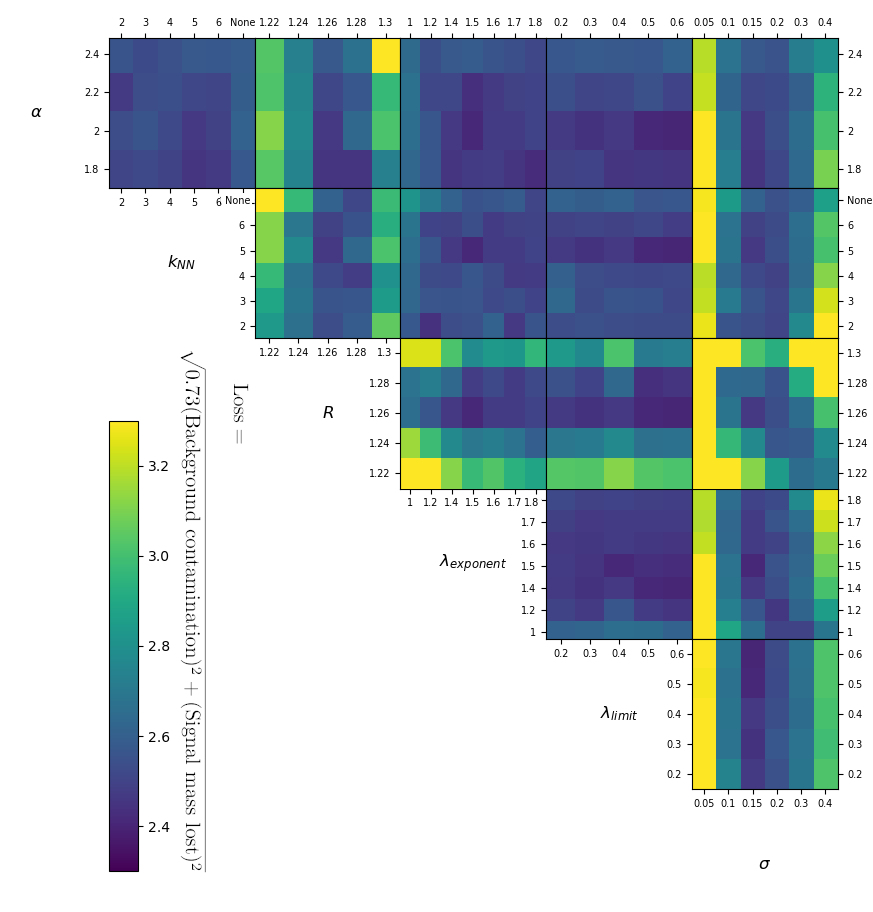
\includegraphics[width=1\textwidth]{graphics/trangle_scan_incomplete.png}
            \caption{There are 5 free parameters for spectral clustering,
                as described in section~\ref{sec:spectralmethodparam}.
                Here the loss, as described in equation~\ref{eqn:loss}, is shown for reasonable of parameter ranges.
                These ranges are either chosen by convention (e.g. \(\alpha\) is conventionally \(1\) or \(2\))
                or chosen according to physical scales (e.g. the distance between particles is of order \(0.1\),
                so \(\sigma\) should be of the same order).
                It can be seen that some parameters, such as \(\alpha\), \(k_\text{NN}\), \(\lambda_\text{exponent}\)
                and \(\lambda_\text{limit}\) are relatively insensitive.
                They give good results in a wide range of values.
                By contrast \stoppingdeltar{} and \(\sigma\) must fall in a narrow range to yield good results.
                {\color{red}TODO; Get data/clip to fill in white space.}
             }\label{fig:scan_spectral}
    \end{figure}    


    The parameters used in the remained of this work are \(\alpha=2.\), \(k_\text{NN}=5\), \(\stoppingdeltar{} = 1.26\), \(\lambda_\text{exponent} = 1.4\) and \(\lambda_\text{limit} = 0.4\).
\subsubsection{Particle data}

    In order to evaluate the behaviour of this clustering method three datasets are used.

    \begin{enumerate}
        \item A \(125\)GeV simulated Higgs cascade decay.
    One Standard Model (SM) Higgs at \(125\)GeV decays to two light Higgs at \(40\)GeV,
    which in turn decay to \beau{}-\bbar{} quark pairs.
    That is \(p^+ p^+ \rightarrow H_{125\text{GeV}} \rightarrow h_{40\text{GeV}} h_{40\text{GeV}} \rightarrow \beau \bbar \beau \bbar\).

     \item The second dataset used is a \(500\)GeV simulated Higgs cascade decay.
         One Heavy Higgs, from the two Higgs doublet model, type-II~\cite{2hdm_modelfile}, at \(500\)GeV decays to two SM Higgs at \(125\)GeV,
    which in turn decay to \beau{}-\bbar{} quark pairs.
    That is \(p^+ p^+ \rightarrow H_{500\text{GeV}} \rightarrow h_{125\text{GeV}} h_{125\text{GeV}} \rightarrow \beau \bbar \beau \bbar\).

    \item For the purpose of checking IRC safety a variety of three jet events are used.
        These jets can be created by any combination of \(g\), \(u\), \(c\), \(d\), \(s\), and their antiparticles.
        It will be generated at leading order and next to leading order.
        This being the simplest possible configuration where IRC singularities could be observed.

     \item {\color{red}TODO; Add ttbar dataset if needed.}

    \end{enumerate}

    Using Madgraph~\cite{alwall_madgraph2011} to generate the partonic process, and Pythia~\cite{sjostrand_pythia2015} to shower, ${\cal O}(10^5)$ of \(pp \rightarrow{} H \rightarrow{} hh \rightarrow{} b\bar{b}b\bar{b}\) events are generated, with $\sqrt{s}=13 $ TeV.


    Both Higgs cascade datasets have the desirable property of creating \bthing{jets} with a range of geometries,
    owing to the boost provided by large mass difference,
    there is a high chance of overlap with 4 \bthing{quarks} in the event.

    Each event also contains some initial state radiation (ISR),
    and from beam remnants.
    ISR is other emissions from the quarks that create the signal process,
    such as radiated gluons.
    Beam remnants are emissions coming from the part of the proton that is not directly involved
    in creating the signal process.



    Before any evaluation can be performed on the final state of the simulation
    particles that ended outside the range of the silicon tracker (\(|\eta|>2.5\))
    or particles with low transverse momentum (\(p_T < 0.5\) GeV) are cut.
    This is to mimic restrictions from reconstruction accuracy.
    These cuts are likely to remove the majority of the radiation from beam remnants,
    and reduce the radiation from ISR.

    %\begin{figure}[htp]
    %    \begin{minipage}[c]{0.5\textwidth}
    %        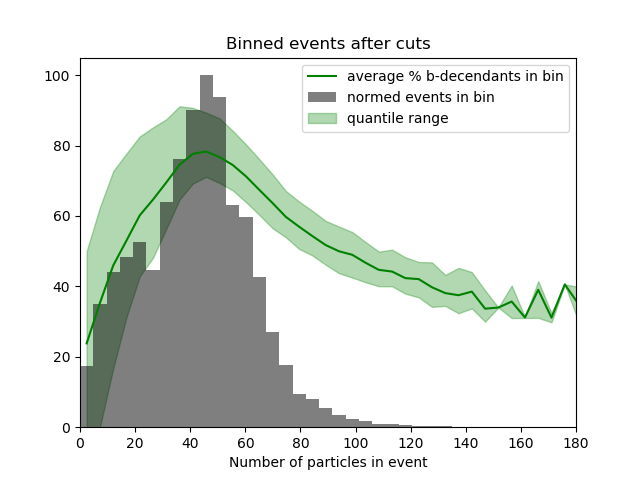
\includegraphics[width=1\textwidth]{graphics/binned_events.png}
    %    \end{minipage}\hfill
    %    \begin{minipage}[c]{0.45\textwidth}
    %        \caption{The end state particles in the simulated events are filtered
    %            with the standard cuts, \(p_T > 0.5\), \(|\eta| < 2.5\).
    %            The events are binned according to how many particles remain after the cuts.
    %            The percentage of \bthing{descendants} in the remaining event after the cuts
    %            is averaged for each bin and plotted on the same axis.
    %            After the cuts have been applied most events are left with around \(50\) particles.
    %                 The percentage of particles that are descendant from a \bthing{quark} varies,
    %                 it is at its highest in events with \(50\) particles,
    %             and most variable in events will small multiplicity.
    %            Very large and very small events tend to be mostly background,
    %            mid sized events are mostly signal.
    %         }\label{fig:bdecendantpercent}
    %    \end{minipage}
    %\end{figure}    
    %
    %
    %\begin{figure}[htp]
    %    \begin{minipage}[c]{0.5\textwidth}
    %        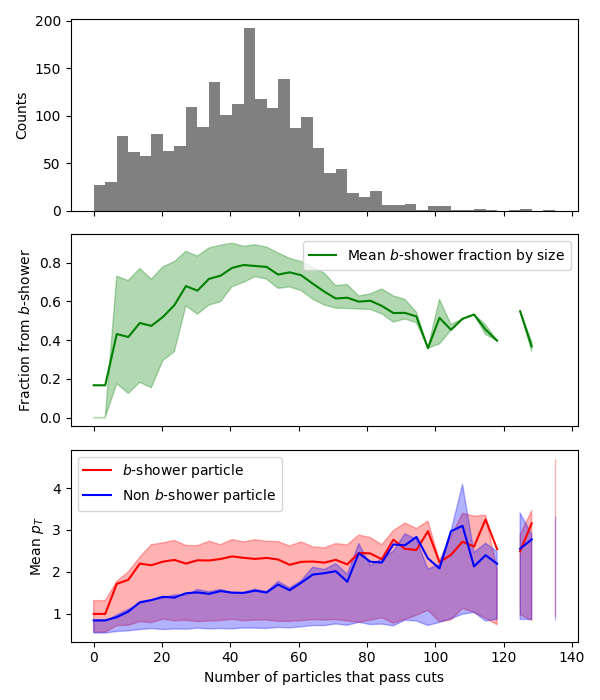
\includegraphics[width=1\textwidth]{graphics/event_composition.png}
    %    \end{minipage}\hfill
    %    \begin{minipage}[c]{0.45\textwidth}
    %        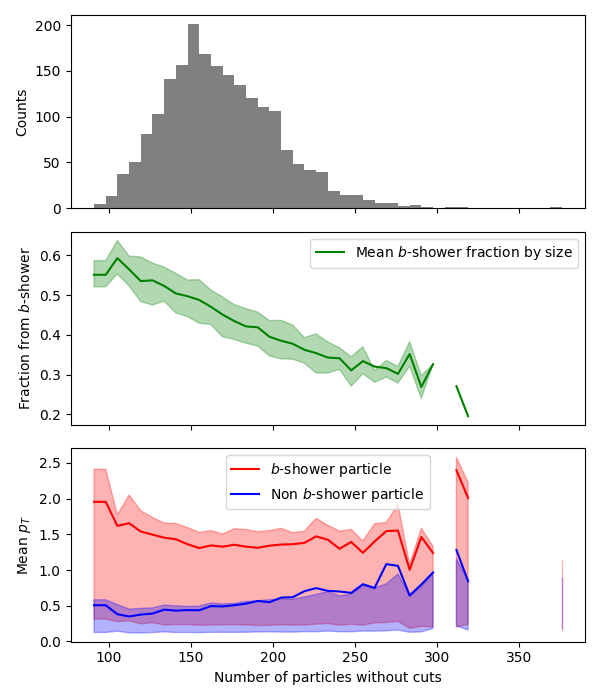
\includegraphics[width=1\textwidth]{graphics/event_composition_nocuts.png}
    %        \caption{Left = with cuts, right = without cuts.
    %         }
    %    \end{minipage}
    %\end{figure}    
    %
    %
    %\begin{figure}[htp]
    %    \begin{minipage}[c]{0.5\textwidth}
    %        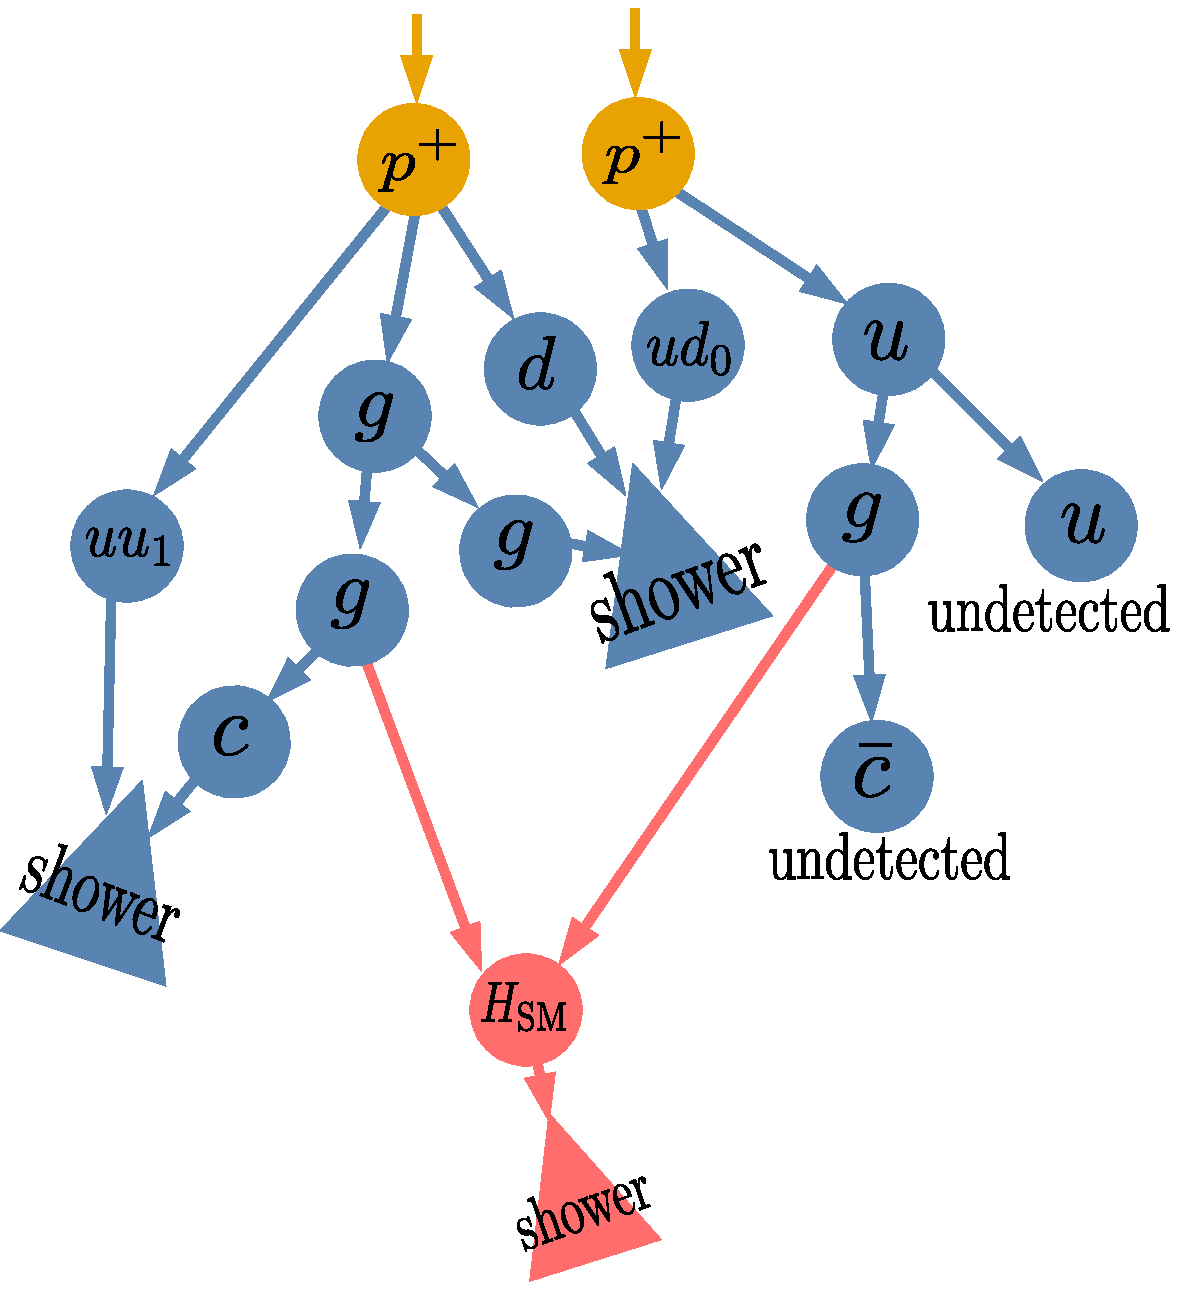
\includegraphics[width=1\textwidth]{graphics/event6.pdf}
    %    \end{minipage}\hfill
    %    \begin{minipage}[c]{0.45\textwidth}
    %        \caption{Drawing of initial state radiation of the 6th even in the dataset.
    %                 The Monte Carlo simulation considers multiple interactions in each vertex,
    %                 and so vertices should eb seen as the combination of multiple steps.
    %                 The information displayed here is what is recorded in the \lstinline{.hepmc} file
    %                 produced by \lstinline{Delphes}.
    %                 A gluon coming from the \(u\) in the left proton producing radiation (the \(c\) and \(g\)) leads to detectable showers.
    %                 The up quark from the right hand proton would have created a shower, but the shower is undetected, either due to high rapidity or low \(p_T\).
    %             Showers are often contributed to from many parts of the initial state radiation, so attributing them has some ambiguity.}
    %        \label{fig:isr}
    %%        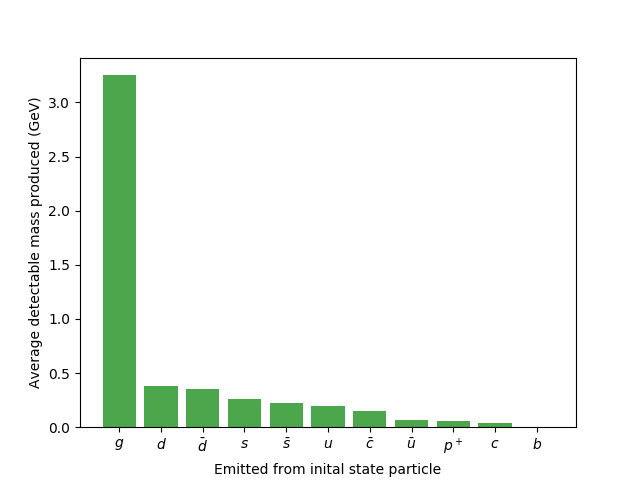
\includegraphics[width=1\textwidth]{graphics/initalstaterdiation_sources.png}
    %%        \caption{In the plot the energy of the initial state particle is used to guess its contribution to the mass of the resulting shower.
    %%            This is done after detector cuts (particle \(p_T > 0.5\) and \(|\text{rapidity}| < 2.5\))
    %%        Taking this rule, on average each event has about \(3\)GeV worth of radiation from initial state gluons.
    %%        Other initial state particles contribute smaller amounts of radiation.}
    %%                 
    %    \end{minipage}
    %\end{figure}    
    %A particle is considered a \bthing{descendant} if it is found in the chain of decays from a \bthing{quark},
    %as opposed to decaying from the ISR.
    After cuts, \(72\%\) of events have at least \(5\) \bthing{shower} particles and \(5\) pure ISR shower particles available.
    These ISR components add noise to the data.
    %Exactly how the percentage of \bthing{descendants} changes with event size is visualised in figure~\ref{fig:bdecendantpercent}.

\subsubsection{Determining IRC safety}\label{sec:IRCmethod}
    It would be possible to demonstrate IRC safety analytically, however,
    as the environment required for clustering on Monte Carlo data is already set up
    it is more efficient for this study to prove IRC safety with data.
    This can be done by showing that an IRC sensitive variable, for example the jet mass spectrum,
    is stable between a leading order (LO) dataset with no IRC singularities and a next to leading order (NLO)
    dataset which will contain IRC singularities.

    Showing the jet mass spectrum at LO and NLO for a particular configuration,
    that is a particular selection of clustering parameters,
    would allow a comparison that would highlight any differences cause by IRC sensitivity.
    This will be done for illustrative purposes,
    however, event an IRC unsafe algorithm such as Iterative Cone~\cite{cacciari_antikt2018}
     has some configurations for which it these singularities are avoided.

    To provided a more global view a scan of parameter configurations must be compared.
    Thus, for an unsafe algorithm (such as Iterative Cone) the unsafe configuration
    will be found.
    It would be cumbersome to compare all these jet mass spectrum by eye, however.
    Instead we introduce a summery statistic representing the divergence between two distributions,
    the Jenson Shannon score~\cite{jensen_shannon}.

    The Jenson Shannon score is a value computed between two distributions that increases in magnitude the more these distributions differ.
    It is a symmetrized variant of the Kullback-Leibler divergence.
    The Kullback-Leibler divergence between probability densities \(p\) and \(q\) can be written;
    \[D_\text{KL} (p | q) = \int^{\inf}_{-inf} p(x) log\left(\frac{p(x)}{q(x)}\right) dx.\]
    From which the Jenson Shannon divergence can be written;
    \[D_\text{JS}(p, q) = \frac{1}{2}D\left(p | \frac{1}{2}(p + q)\right) + \frac{1}{2}D\left(q | \frac{1}{2}(p + q)\right)\]
    \(D_\text{JS}\) treats \(p\) and \(q\) symmetrically, and will grow as they become more different.
    The spectrum of Jenson Shannon scores will be plotted for a known IRC safe clustering algorithm, Anti-kt,
    a known unsafe clustering algorithm Iterative Cone and the spectral clustering algorithm.

    One small issue with this method is that a large \(D_\text{JS}\) would not differentiate
    between a change in \(p\) and \(q\) due to IRC sensitivity and 
    a change due to noise in the jet mass spectrum.
    The more events used to find the jet mass spectrum the lower the expected noise,
    however is is also possible to subsample within a distribution (LO or NLO)
    to discover how much \(D_\text{JS}\) is influenced by noise.
    If two random sets of jet masses, from events \(a\) and events \(b\) are drawn from the LO events,
    and a \(D_\text{JS}(a, b)\) is computed between them, a large value will indicate that 
    noise in the spectrum is increasing the size of \(D_\text{JS}\) between the LO and NLO spectrums.
    To account for this a subsampled \(D_{JS}\) can be constructed;
    \[D_{JS, subsampled}(p, q) = \frac{cD_{JS}(p, q)}{\sum_{a \in p, b \in p} D_{JS}(a, b)\sum_{c \in q, b \in q} D_{JS}(c, d)}\]
    If this does not differ too much from \(D_{JS}\) then the data sets are large enough the noise in
    the spectrum is not influencing the results.
